\section{Aplicaciones}

% %------------------------------------------------ aplicaion 1 -------------------------------------------
% \subsection{Modelo del transporte}
% 
% Este modelo se usa para describir un problema de programaci\'on sobre el transporte de insumos, personas, etc. desde lugares de origen a 
% determinados destinos. Los modelos sirven, entre otras cosas, para la toma decisiones sobre planificaci\'on, ingenierı\'ia, adquisici\'on de 
% veh\'iculos de transporte, capacidad de infraestructura, impactos ambientales, contaminaci\'on, etc.\\ 
% 
% Veamos un ejemplo de una situaci\'on que se estudia con este modelo.\\
% Supongamos que tenemos $m$ centros de suministro, de donde podemos transportar ciertos insumos a $n$ destinos.\medskip 
% 
% $a_i: $ el n\'umero de unidades disponibles de un producto del lugar de suministro $i,\,\,i=1,\, \ldots \, , m.$\\
% $b_j: $ el n\'umero de unidades de determinado producto con que se desea abastacer el destino $j,\,\, j=1,\, \ldots \, , n. $\\
% $C_{ij} $ el costo para transportar una unidad del producto desde el origen $i$ hasta el destino $j,$ con  $i=1,\, \ldots \, , m;
% \,\,\, j=1,\, \ldots \, , n.$
% \medskip
% 
% El problema consiste determinar el n\'umero de unidades del producto que se debe transportar de cada lugar de suministro a cada destino, de 
% manera que el costo total sea m\'inimo y se cumplan con los niveles de disponibilidad de cada origen y de requerimiento de cada destino. De 
% esta manera se debe:
% 
% \begin{eqnarray*}
%    \mbox{maximizar } & z = \displaystyle{\sum_{i,j = 1}^{m,n} C_{ij}x_{ij}} &  \\
%    \mbox{sujeto a  } & \displaystyle{\sum_{j = 1}^{n}} x_{ij}  \leqslant a_i; & i=1,\, \ldots \, , m\\
%    &  \displaystyle{\sum_{i = 1}^{m}} x_{ij}\geqslant b_j & j=1,\, \ldots , , n\\
%    &  x_{ij} \geqslant 0 & i=1,\, \ldots \, , m.\,\, j=1,\, \ldots \, , n
% \end{eqnarray*}
% 
% donde $x_{ij},\,\, i=1,\, \ldots \, , m.\,\, j=1,\, \ldots \, , n $ representan el n\'umero de unidades que se han de transportar desde el 
% lugar $i$ al destino $j.$ Para la resoluci\'on de estos problemas se usan ciertos m\'etodos como: el de la {\it esquina noroeste, costo
% m\'inimo y de la aproximaci\'on de Vogel}\\ \\
% \
% %--------------------------------------------fin--------------------------------------------------------------------------------------

%--------------------------------------------portafolio-------------------------------------------------------------------------------------
\subsection{El problema del portafolio \cite{intro}}

El problema cl\'asico de optimizaci\'on de portafolio, en el que un agente escoge sus estrategias a modo de maximizar su utilidad esperada 
ha sido estudiado en profundidad por mucho tiempo. Sin embargo, solo hace poco ha surgido el inter\'es por plasmar el hecho de que la 
selecci\'on de un modelo particular al momento de hacer la toma de decisiones es en s\'i riesgosa.
\medskip

El problema del portafolio se define de la siguiente manera:

\begin{eqnarray*}
   \min & \dfrac{1}{2} x^{t} \sum x +  r^{t} x &  \\
   \mbox{sujeto a } & \sum x_i =1 & x_i \geqslant 0
\end{eqnarray*}

donde $ \sigma \in \mathbb{R}^{n \times n} $ es la matriz de varianza covarianza y $ r \in \mathbb{R}.$ El problema del portafolio puede ser
convertido al siguiente problema:

\begin{eqnarray*}
   \min & \dfrac{1}{2} x^{t} \sum x +  r^{t} x + \mathbb{I}_{C} & 
\end{eqnarray*}

donde $\mathbb{I}_{C}$ es la funci\'on indicadora del conjunto $C = \{x \in \mathbb{R}^{n}|\, \sum x_i = 1. x_i \geqslant 0 \}.$ Se puede
aplicar el m\'etodo del gradiente pr\'oximo si se calcula el operador pr\'oximo de la funci\'on indicadora $\mathbb{I}_{C}.$ 

{\definicion \textbf{\itshape (Operador pr\'oximo)} Sea $f: \mathbb{R}^n \longmapsto [-\infty,\, +\infty)$ una funci\'on propia, convexa y 
cerrada. Se define el operador pr\'oximo $prox_{f}:  \mathbb{R}^n \longmapsto  \mathbb{R}^n $ de $f $ como 
\begin{equation}
   proy_{f}(v) = \arg \min_{x} \{f(x) + \dfrac{1}{2} ||x - v||^2\}
\end{equation}
donde $|| \cdot ||$ es la norma euclidiana. \label{operador_proximo} }~
\medskip

Dada la definici\'on(\ref{operdor_proximo}), $prox_{f}(v) $ es un punto que se encuentra entre $x^* = \min\{f\} $ y cerca de $v.$ Cuando $f$
es la funci\'on indicadora de $C \subseteq \mathbb{R}^n $ es decir

\[\mathbb{I}_C (x) = \left \{ \begin{array}{rcl}
                                 0 & x \in C & \\
                                  &  &  \\
                                 +\infty  & x \notin C & 
                              \end{array}
\right. \]


entonces \begin{equation}
           prox_{f}(v) = \arg \min_{x \in C} \{|| x - v || \} 
           \label{proy_general}
         \end{equation}

As\'i el operador pr\'oximo se puede ver como una proyecci\'on generalizada.

Usando (\ref{proy_general}) se puede obtener \'este operador conociendo como se proyecta sobre el conjunto $C$.
La proyección sobre el conjunto C $C.$ La proyecci\'on sobre el conjunto $C$ est\'a dada por:

\[ \prod_{C}(v) = \max {v_i - \mu^{*}, 0} \]

Donde $\mu$ es la ra\'iz de la funci\'on

\[ f = \sum_{i = 1}^{n} \max{v_i - \mu, 0} - 1 \]

Utilizando (lo que falta), el operador pr\'oximo de $\mathbb{I}_{C}$ est\'a dada por 
$$\mbox{proy}_{\mathbb{I}_{C}}(v) = \max{v_i - \mu^{*}, 0}$$

\textbf{Ejemplo \cite{intro}}\medskip

Sea $ P^{1}, \ldots , p^{5} $ los precios de cinco empresas de rama de construcci\'on: Se tomaron los datos del $ 2009 \,- \, 2014 $ de los 
precios diarios de las acciones. Los rendimientos diraios de la empresa $i$ est\'an dados por $r_{i}^{j} = \ln,\left(\dfrac{P_{j + 1}^{i}}
{P_j}\right).$
$\sigma $ es la matriz de varianza covarianza muestral\\

$$\sigma = \begin{pmatrix}
             0.0000778 & 0.00000796 & 0.000000645 & 0.0000541 & 0.00000346 \\
             0.00000796 & 0.000512  & −0.0000432  & 0.0000551 & 0.00000273 \\
             0.000000645 & −0.0000432 & 0.000315  & 0.000305  & 0.0000149 \\
             0.0000541   & 0.0000551  & 0.000305  & 0.0043    & 0.000116\\
             0.00000346  & 0.00000273 & 0.0000149 & 0.000116  & 0.000208
          \end{pmatrix}
$$

y el vector $\vec{r} $ es la media muestral de los rendimientos de cada empresa
\[\vec{r} = (−0.0004142, 0.0004127, 0.0018, −0.00411, 0.0008422)\]

aplicando el m\'etodo del gradiente pr\'oximo se lleg\'o al punto
\[x^{*} = (0, 0, 0.9999, 0, 0)\]

en diez iteraciones, en un tiempo de $0.2140$ segundos. Lo que significa que todod el dinero se debe invertir en la acci\'on de la empresa 
$3.$
%--------------------------------------------fin--------------------------------------------------------------------------------------


%---------------------------------------  imagenes  ----------------------------------------------------------------------------------
\subsection{Procesamiento de im\'agenes: Transformada distancia \cite{lara}.}

En procesamiento de im\'agenes, la tranformada distancia, tiene diversas aplicaciones, por ejemplo, en medicina, visualizaci\'on de
estructuras o im\'agenes geom\'etricas \cite{lara}. %ver referencias
\medskip

Para una imagen binaria $B$ definida como una aplicaci\'on de $\{1, \ldots , n\} \times \{1, \ldots , m\} $ a $ \{0, 1\},$ la transformada
distancia es la funci\'on que asocia $B$ con un {\it array $ D $} de la forma $ \{1, \ldots , n\} \times \{1, \ldots , m\} $ a $ \{0, 1\},$
definida como: Asumimos que $B$ tiene al menos un pixel $p$ con $B[p] = 0.$ Para cada pixel $ p $ en $ B,\ D[p] $ contiene la distancia 
eucl\'idea al pixel m\'as cercano en $ B $ que contiene el valor $0.$ En la pr\'actica, para restringir la computaci\'on aritm\'etica entera,
la transformada distancia $ D^2 $ es calculada\\ 

$$B = \begin{bmatrix}
   1 & 1 & 1 & 1 & 1\\
   1 & 0 & 1 & 1 & 1\\
   1 & 1 & 1 & 1 & 1\\
   1 & 1 & 1 & 0 & 1\\
   1 & 1 & 1 & 1 & 1
\end{bmatrix} \,\,\,\,\,\mbox{    es    }\,\,\,\,\,\,\,
D^2 =
\begin{bmatrix}
   2 & 1 & 2 & 5 & 8\\
   1 & 0 & 1 & 4 & 5\\
   2 & 1 & 2 & 1 & 2 \\
   5 & 4 & 1 & 0 & 1\\
   8 & 5 & 2 & 1 & 2
\end{bmatrix}
$$
~\\

Varios algoritmos han sido introducidos para calcular la transformada distancia (Euclidean Distance Transform) \'o EDT. Recientes 
investigaciones se centran en simplificar los algoritmos aun alcanzando complejidad de tiempo lineal. Por ejemplo, el hecho que la
computaci\'on de la EDT es equivalente a calcular la menor envoltura de funciones cuadr\'aticas y con ello se present\'o un algoritmo de
complejidad lineal. Otros algoritmos basados en la monotonicidad o propiedades de vecindad son manejados para alcanzar tambi\'en complejidad
lineal.\\\\

La relaci\'on entre la envoltura de Moreau y la conjugada de Fenchel-Legendre para reducir el c\'alculo de la transformada distancia usando 
el algoritmo LLT es esencia, como sigue:\\ \\

El cuadrado de la transformada distancia es la aplicaci\'on $ D^2 $ desde $ \{1, \ldots , n\} \times \{1, \ldots , m\} $ al conjunto de 
enteros no negativos definidos por 

\[D^2(p) = \min_{q \in O} \parallel p - q \parallel^2\]

D\'onde $ O = \{q:\, B(q) = 0\} $ es el conjunto de pixeles con valor $0$ en $B.$ Usando la funci\'on indicador $ I(p) = 0 $ si $ B(p) = 0 $
y $ \infty $ en otros casos, podemos encontrar el cuadrado de la transformada distancia de Moreau de $I$

\[D^2(p) = \min_{q \in O} \parallel p - q \parallel^2 + I(q)\]


As\'i los algoritmos para la transformada distancia son casos particulares de los algoritmos para calcular la envoltura de Moreau.\\ \\

Ejemplos de aplicaciones basadas en transformadas de distancia incluyen la morfometr\'ia de los nervios transversales, el registro de
im\'agenes de resonancia magn\'etica, c\'amara de ruta de planificaci\'on en endoscopia virtual y clasificaci\'on de tejidos en las 
im\'agenes de resonancia magn\'etica.\medskip
% continuar ma\~nana

La siguiente figura basada en el \textbf{algoritmo PE} muestra la transformada distancia de una imagen binario con la distancia cuadrada
Euclı́dea.

\begin{itemize}
   \item \ref{imagen}(a) muestra la imagen de entrada.
   \item La transformación de la entrada a lo largo de cada columna se muestra en \ref{imagen}(b).
   \item La transformada distancia final, obtenida mediante la transformación del resultado intermedio a lo largo de cada fila, se muestra 
	 en \ref{imagen}(c).
\end{itemize}

Los p\'íxeles oscuros corresponden a valores bajos mientras que los p\'ixeles brillantes corresponden a valores altos.

\begin{figure}[h]
  \centering
  \subfigure[]{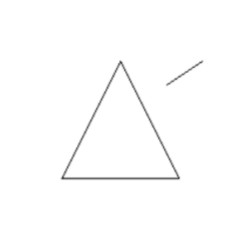
\includegraphics[scale = 0.5]{./partes/sub_sec/entrada1.jpg}}
  \subfigure[]{
\includegraphics[scale = 0.5]{./partes/sub_sec/entrada2.jpg}}
  \subfigure[]{
\includegraphics[scale = 0.5]{./partes/sub_sec/entrada3.jpg}}
  \caption{Transformada distancia de una imagen binario con la distancia cuadrada Euclı́dea}
  \label{imagen}
\end{figure}
%-------------------------------------- fin --------------------------------------------------------------------------------------

%\subsection{pendiente}










